\documentclass[10pt,landscape,letter]{article}
\usepackage[landscape,margin=0.5in]{geometry}
\usepackage{multicol}
\usepackage{amsmath,amssymb}
\usepackage{graphicx}
\usepackage{xcolor}
\usepackage{tikz}
\usepackage{booktabs}
\usepackage{enumitem}
\usepackage{fancyhdr}
\usepackage{titlesec}
\usepackage{fancyvrb}

% Compact formatting
\setlength{\parindent}{0pt}
\setlength{\parskip}{2pt}
\setlist[itemize]{leftmargin=*, noitemsep, topsep=0pt}
\setlist[enumerate]{leftmargin=*, noitemsep, topsep=0pt}

% Section formatting
\titleformat{\section}{\normalfont\normalsize\bfseries\color{blue!70!black}}{\thesection}{0.5em}{}
\titleformat{\subsection}{\normalfont\small\bfseries\color{blue!50!black}}{\thesubsection}{0.5em}{}
\titlespacing*{\section}{0pt}{4pt}{2pt}
\titlespacing*{\subsection}{0pt}{3pt}{1pt}

% Box for important formulas
\newcommand{\importantbox}[1]{%
  \fcolorbox{blue!50!black}{blue!5}{%
    \parbox{0.95\linewidth}{#1}%
  }%
}

% Highlight color
\newcommand{\highlight}[1]{\colorbox{yellow!30}{$#1$}}

%\pagestyle{fancy}
%\fancyhf{}
%\fancyhead[C]{\raisebox{-8pt}{\textbf{Branched and Cyclic Pathways -- Cheat Sheet V1.0}}}
%\fancyfoot[C]{\thepage}
%\renewcommand{\headrulewidth}{0.5pt}

\pagestyle{fancy}
\fancyhf{}
\fancyhead[C]{\raisebox{-10pt}{\textbf{Transfer Functions \& Control in Biochemical Networks -- Cheat Sheet V1.0}}\\[-10pt]}
\fancyfoot[C]{\thepage}
\renewcommand{\headrulewidth}{0.5pt}

\begin{document}

\begin{multicols}{3}

% =============================================================================
\section{Fundamental Equations}
% =============================================================================

\subsection{Mass Balance ODE}
\begin{equation*}
\frac{d\mathbf{S}}{dt} = \mathbf{N} \cdot \mathbf{v}(\mathbf{S}, \mathbf{p})
\end{equation*}
\begin{itemize}
\item $\mathbf{S}$ = concentration vector (species)
\item $\mathbf{N}$ = stoichiometry matrix
\item $\mathbf{v}$ = rate vector (fluxes)
\item $\mathbf{p}$ = parameter vector
\end{itemize}

\subsection{Stoichiometry Matrix Properties}
\begin{itemize}
\item Rows = species ($m$), Columns = reactions ($r$)
\item Rank($\mathbf{N}$) = $m_0$ = \# independent species
\item $m - m_0$ = \# conservation relations
\end{itemize}

\subsection{Steady State}
At steady state: $\mathbf{N} \cdot \mathbf{v}^0 = \mathbf{0}$

% =============================================================================
\section{Stoichiometric Analysis}
% =============================================================================

\subsection{Null Spaces of N}

\textbf{Right null space} (kernel):
\begin{equation*}
\mathbf{N} \cdot \mathbf{K} = \mathbf{0}
\end{equation*}
\begin{itemize}
\item Columns of $\mathbf{K}$ = steady-state flux vectors
\item Dimension = $r - m_0$ = degrees of freedom
\item Any steady-state flux: $\mathbf{v}^{ss} = \mathbf{K} \cdot \boldsymbol{\alpha}$
\end{itemize}

\textbf{Left null space}:
\begin{equation*}
\mathbf{G} \cdot \mathbf{N} = \mathbf{0}
\end{equation*}
\begin{itemize}
\item Rows of $\mathbf{G}$ = conservation relations
\item Dimension = $m - m_0$
\item Conserved quantity: $\mathbf{G} \cdot \mathbf{S} = \mathbf{T}$ (constant)
\end{itemize}

\subsection{The Link Matrix L}

Partition species into \textbf{independent} ($\mathbf{S}_i$) and \textbf{dependent} ($\mathbf{S}_d$):
\begin{equation*}
\mathbf{S} = \begin{pmatrix} \mathbf{S}_i \\ \mathbf{S}_d \end{pmatrix}
\end{equation*}

The \textbf{link matrix} $\mathbf{L}$ relates them:

$\mathbf{S} = \mathbf{L} \mathbf{S}_i + \mathbf{T}$, where
$\mathbf{L} = \begin{pmatrix} \mathbf{I} \\ \mathbf{L}_0 \end{pmatrix}$

\begin{itemize}
\item $\mathbf{L}_0$ = $(m-m_0) \times m_0$ matrix
\item $\mathbf{T}$ = conserved totals vector
\item $\mathbf{L}_0$ comes from row reduction of $\mathbf{N}$
\end{itemize}

\subsection{Reduced Stoichiometry Matrix}

\importantbox{
\begin{equation*}
\mathbf{N} = \mathbf{L} \cdot \mathbf{N}_r
\end{equation*}
}
\begin{itemize}
\item $\mathbf{N}_r$ is $m_0 \times r$ (full row rank)
\item Rows correspond to independent species only
\item Reduced system: $\dfrac{d\mathbf{S}_i}{dt} = \mathbf{N}_r \cdot \mathbf{v}$
\end{itemize}

\subsection{Relationships Between Matrices}
\begin{align*}
\mathbf{N} &= \mathbf{L} \cdot \mathbf{N}_r \\
\mathbf{G} \cdot \mathbf{L} &= \mathbf{0} \\
\mathbf{L}^T \cdot \mathbf{G}^T &= \mathbf{0}
\end{align*}

\subsection{Computing L from N}

\textbf{Method:} Row reduce $\mathbf{N}$ to row echelon form
\begin{enumerate}
\item Identify pivot columns $\rightarrow$ independent species
\item Non-pivot rows give $\mathbf{L}_0$
\item $\mathbf{L} = \begin{pmatrix} \mathbf{I} \\ \mathbf{L}_0 \end{pmatrix}$
\end{enumerate}

\subsection{Example: Conserved Cycle}

\begin{center}
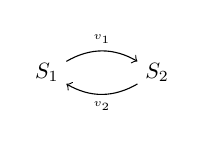
\begin{tikzpicture}[scale=0.7, every node/.style={scale=0.8}]
\node (S1) at (0,0) {$S_1$};
\node (S2) at (2,0) {$S_2$};
\draw[->, bend left=30] (S1) to node[above]{\tiny $v_1$} (S2);
\draw[->, bend left=30] (S2) to node[below]{\tiny $v_2$} (S1);
\end{tikzpicture}
\end{center}

Stoichiometry matrix:
\begin{equation*}
\mathbf{N} = \begin{pmatrix} -1 & 1 \\ 1 & -1 \end{pmatrix} \quad \text{rank} = 1
\end{equation*}

\begin{itemize}
\item One independent species (e.g., $S_1$)
\item Conservation: $S_1 + S_2 = T$ (constant)
\end{itemize}

\textbf{Link matrix:}
\begin{equation*}
\mathbf{L} = \begin{pmatrix} 1 \\ -1 \end{pmatrix}, \quad \mathbf{L}_0 = (-1)
\end{equation*}

So $S_2 = -S_1 + T = T - S_1$

\textbf{Reduced system:}
$\mathbf{N}_r = (-1 \quad 1)$

$\dfrac{dS_1}{dt} = -v_1 + v_2$

\subsection{The K Matrix (Kernel)}

$\mathbf{K}$ spans all possible steady-state fluxes:
\begin{equation*}
\mathbf{v}^{ss} = \mathbf{K} \cdot \mathbf{j}
\end{equation*}
where $\mathbf{j}$ = vector of independent fluxes

\textbf{Computing K:}
\begin{enumerate}
\item Row reduce $\mathbf{N}^T$
\item Identify free variables
\item Express basic variables in terms of free
\item Columns of $\mathbf{K}$ = basis vectors
\end{enumerate}

\textbf{Dimension check:}
\begin{equation*}
\dim(\mathbf{K}) = r - \text{rank}(\mathbf{N}) = r - m_0
\end{equation*}

\subsection{Example: Branched Pathway}

\begin{center}
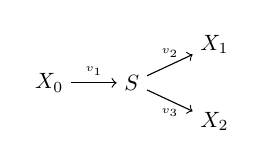
\begin{tikzpicture}[scale=0.7, every node/.style={scale=0.8}]
\node (X0) at (0,0) {$X_0$};
\node (S) at (1.5,0) {$S$};
\node (X1) at (3,0.7) {$X_1$};
\node (X2) at (3,-0.7) {$X_2$};
\draw[->] (X0) -- node[above]{\tiny $v_1$} (S);
\draw[->] (S) -- node[above]{\tiny $v_2$} (X1);
\draw[->] (S) -- node[below]{\tiny $v_3$} (X2);
\end{tikzpicture}
\end{center}

$X_0, X_1, X_2$ = external (fixed); $S$ = internal variable

Stoichiometry matrix:
\begin{equation*}
\mathbf{N} = \begin{pmatrix} 1 & -1 & -1 \end{pmatrix} \quad (1 \times 3)
\end{equation*}

\begin{itemize}
\item rank$(\mathbf{N}) = 1$, so $\dim(\mathbf{K}) = 3 - 1 = 2$
\end{itemize}

\textbf{Kernel matrix:}
\begin{equation*}
\mathbf{K} = \begin{pmatrix} 1 & 1 \\ 1 & 0 \\ 0 & 1 \end{pmatrix}
\end{equation*}

Columns represent independent flux patterns:
\begin{itemize}
\item $(1,1,0)^T$: flux through branch 1
\item $(1,0,1)^T$: flux through branch 2
\end{itemize}

Any steady-state flux: $\mathbf{v} = \alpha \begin{pmatrix}1\\1\\0\end{pmatrix} + \beta \begin{pmatrix}1\\0\\1\end{pmatrix}$

At steady state: $v_1 = v_2 + v_3$ (branch point balance)

% =============================================================================
\section{Elementary Modes}
% =============================================================================

\subsection{Definition}
An \textbf{elementary mode (EM)} is a minimal set of reactions that can operate at steady state.

\importantbox{
\textbf{Properties:}
\begin{itemize}
\item Satisfies $\mathbf{N} \cdot \mathbf{e} = \mathbf{0}$
\item Non-decomposable (no subset is valid)
\item Unique up to scaling
\end{itemize}
}

\subsection{Relation to K Matrix}
\begin{itemize}
\item Columns of $\mathbf{K}$ span the flux space
\item EMs are the \textit{edges} of the flux cone
\item Every steady-state flux is a non-negative combination of EMs (for irreversible reactions)
\end{itemize}

\subsection{Elementary Mode Matrix E}
\begin{equation*}
\mathbf{N} \cdot \mathbf{E} = \mathbf{0}
\end{equation*}
Each column of $\mathbf{E}$ is an elementary mode.

Any feasible flux:
\begin{equation*}
\mathbf{v} = \mathbf{E} \cdot \boldsymbol{\omega}, \quad \boldsymbol{\omega} \geq \mathbf{0}
\end{equation*}

\subsection{Flux Cone Geometry}
\begin{center}
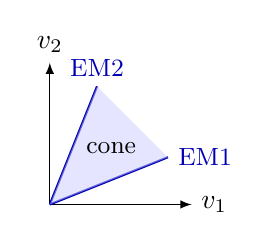
\begin{tikzpicture}[scale=0.6]
\draw[-latex] (0,0) -- (3,0) node[right] {$v_1$};
\draw[-latex] (0,0) -- (0,3) node[above] {$v_2$};
\draw[thick, blue!70!black] (0,0) -- (2.5,1) node[right] {\small EM1};
\draw[thick, blue!70!black] (0,0) -- (1,2.5) node[above] {\small EM2};
\fill[blue!20, opacity=0.5] (0,0) -- (2.5,1) -- (1.75,1.75) -- (1,2.5) -- cycle;
\node at (1.3,1.2) {\small cone};
\end{tikzpicture}
\end{center}
\begin{itemize}
\item EMs define edges of the cone
\item Interior points = combinations of EMs
\item Reversible reactions: cone becomes subspace
\end{itemize}

\subsection{Finding Elementary Modes}

\textbf{Simple cases:} Inspect network for minimal cycles

\textbf{Algorithm (conceptual):}
\begin{enumerate}
\item Start with null space basis $\mathbf{K}$
\item Find extreme rays of $\{\mathbf{v}: \mathbf{N}\mathbf{v}=0, \mathbf{v}\geq 0\}$
\item Each extreme ray = one EM
\end{enumerate}

\textbf{Software:} \texttt{efmtool}, \texttt{metatool}, \texttt{COPASI}

\subsection{Biological Interpretation}
\begin{itemize}
\item EMs = ``pathways through the network''
\item Each EM is a functional unit
\item Cell uses weighted sum of EMs
\item Minimal: removing any reaction breaks it
\end{itemize}

\subsection{Example: Linear Pathway}
\begin{center}
$X_0 \xrightarrow{v_1} S_1 \xrightarrow{v_2} S_2 \xrightarrow{v_3} X_1$
\end{center}
\begin{itemize}
\item $\mathbf{N} = \begin{pmatrix} 1 & -1 & 0 \\ 0 & 1 & -1 \end{pmatrix}$
\item Only one EM: $\mathbf{e} = (1, 1, 1)^T$
\item All fluxes equal at steady state
\end{itemize}

\subsection{Example: Branched Pathway}
\begin{center}
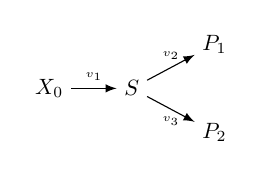
\begin{tikzpicture}[scale=0.7, every node/.style={scale=0.8}]
\node (X0) at (0,0) {$X_0$};
\node (S) at (1.5,0) {$S$};
\node (P1) at (3,0.8) {$P_1$};
\node (P2) at (3,-0.8) {$P_2$};
\draw[-latex] (X0) -- node[above]{\tiny $v_1$} (S);
\draw[-latex] (S) -- node[above]{\tiny $v_2$} (P1);
\draw[-latex] (S) -- node[below]{\tiny $v_3$} (P2);
\end{tikzpicture}
\end{center}
\begin{itemize}
\item Two EMs: $(1,1,0)^T$ and $(1,0,1)^T$
\item Branch point creates alternatives
\end{itemize}

% =============================================================================
\section{Elasticities}
% =============================================================================

\subsection{Definition}
\textbf{Unscaled elasticity:}
\begin{equation*}
\varepsilon_{ij}^{\text{unscaled}} = \frac{\partial v_i}{\partial S_j}
\end{equation*}

\textbf{Scaled elasticity:}
\begin{equation*}
\boxed{\varepsilon_{ij} = \frac{S_j}{v_i} \cdot \frac{\partial v_i}{\partial S_j} = \frac{\partial \ln v_i}{\partial \ln S_j}}
\end{equation*}

\subsection{Common Elasticity Formulas}

\textbf{Michaelis-Menten:} $v = \frac{V_{\max} S}{K_m + S}$
\begin{equation*}
\varepsilon_S = \frac{K_m}{K_m + S} \quad \text{(ranges 0 to 1)}
\end{equation*}

\textbf{Reversible MM:} $v = \frac{V_f(S/K_S) - V_r(P/K_P)}{1 + S/K_S + P/K_P}$
\begin{align*}
\varepsilon_S &= \frac{1 + P/K_P}{1 + S/K_S + P/K_P} \cdot \frac{v_f}{v} \\
\varepsilon_P &= -\frac{1 + S/K_S}{1 + S/K_S + P/K_P} \cdot \frac{v_r}{v}
\end{align*}

\textbf{Hill kinetics:} $v = \frac{V_{\max} S^n}{K^n + S^n}$
\begin{equation*}
\varepsilon_S = n \cdot \frac{K^n}{K^n + S^n} \quad \text{(ranges 0 to $n$)}
\end{equation*}

\textbf{Mass action:} $v = k \cdot S$
\begin{equation*}
\varepsilon_S = 1
\end{equation*}

\textbf{Inhibition:} $v = \frac{V_{\max} S}{(K_m + S)(1 + I/K_i)}$
\begin{equation*}
\varepsilon_I = -\frac{I/K_i}{1 + I/K_i} \quad \text{(negative, ranges $-1$ to 0)}
\end{equation*}

% =============================================================================
\section{Linearization}
% =============================================================================

\subsection{Taylor Expansion}
Around steady state $(\mathbf{S}^0, \mathbf{v}^0)$:
\begin{equation*}
\frac{d(\delta \mathbf{S})}{dt} = \mathbf{A} \cdot \delta \mathbf{S} + \mathbf{B} \cdot \delta \mathbf{u}
\end{equation*}

\subsection{The Jacobian}
\importantbox{
\begin{equation*}
\mathbf{A} = \mathbf{N} \cdot \boldsymbol{\varepsilon}^{\text{unscaled}}
\end{equation*}
}

\vspace{2pt}
\textbf{Key insight:} Jacobian = Structure $\times$ Local kinetics

\subsection{Jacobian Elements}
\begin{equation*}
A_{ij} = \sum_k N_{ik} \cdot \frac{\partial v_k}{\partial S_j}
\end{equation*}

% =============================================================================
\section{Transfer Functions}
% =============================================================================

\subsection{Laplace Transform}
\begin{equation*}
s \cdot \delta \mathbf{S}(s) = \mathbf{A} \cdot \delta \mathbf{S}(s) + \mathbf{B} \cdot \delta \mathbf{u}(s)
\end{equation*}

\subsection{Transfer Function Definition}
\importantbox{
\begin{equation*}
\mathbf{G}(s) = (s\mathbf{I} - \mathbf{A})^{-1} \mathbf{B}
\end{equation*}
}

\subsection{For 2$\times$2 Systems}
If $\mathbf{A} = \begin{pmatrix} a & b \\ c & d \end{pmatrix}$, then:
\begin{equation*}
(s\mathbf{I} - \mathbf{A})^{-1} = \frac{1}{\Delta(s)} \begin{pmatrix} s-d & b \\ c & s-a \end{pmatrix}
\end{equation*}
where $\Delta(s) = (s-a)(s-d) - bc$

\subsection{Characteristic Polynomial}
\begin{equation*}
\Delta(s) = \det(s\mathbf{I} - \mathbf{A}) = s^2 - \text{tr}(\mathbf{A})s + \det(\mathbf{A})
\end{equation*}

\subsection{Poles and Zeros}
\begin{itemize}
\item \textbf{Poles} = roots of denominator = eigenvalues of $\mathbf{A}$
\item \textbf{Zeros} = roots of numerator
\item Poles determine \textit{stability}
\item Zeros determine \textit{response shape}
\end{itemize}

% =============================================================================
\section{Eigenvalues \& Stability}
% =============================================================================

\subsection{2D System Eigenvalues}
For $\mathbf{A} = \begin{pmatrix} a & b \\ c & d \end{pmatrix}$:
\begin{equation*}
\lambda_{1,2} = \frac{(a+d) \pm \sqrt{(a+d)^2 - 4(ad-bc)}}{2}
\end{equation*}
Or: $\lambda_{1,2} = \frac{\text{tr}(\mathbf{J}) \pm \sqrt{\text{tr}(\mathbf{A})^2 - 4\det(\mathbf{A})}}{2}$

\subsection{Stability Criteria}
\importantbox{
System is \textbf{stable} iff all eigenvalues have $\text{Re}(\lambda) < 0$
}

\vspace{4pt}
\textbf{For 2D systems:}
\begin{itemize}
\item Stable iff $\text{tr}(\mathbf{A}) < 0$ AND $\det(\mathbf{A}) > 0$
\end{itemize}

\subsection{Types of Dynamics}
\begin{center}
\begin{tabular}{ll}
\toprule
Eigenvalues & Behavior \\
\midrule
Real, both $< 0$ & Stable node \\
Real, both $> 0$ & Unstable node \\
Real, opposite signs & Saddle (unstable) \\
Complex, Re $< 0$ & Stable spiral \\
Complex, Re $> 0$ & Unstable spiral \\
Complex, Re $= 0$ & Center (oscillations) \\
\bottomrule
\end{tabular}
\end{center}

\subsection{Time Constants}
\begin{equation*}
\tau_i = -\frac{1}{\text{Re}(\lambda_i)}
\end{equation*}
Largest $\tau$ = slowest mode = dominant dynamics

% =============================================================================
\section{DC Gain \& Control Coefficients}
% =============================================================================

\subsection{The Key Connection}
\importantbox{
\textbf{DC gain} = $\mathbf{G}(0) = -\mathbf{A}^{-1}\mathbf{B}$
\vspace{3pt}

This equals the \textbf{steady-state sensitivity}
}

\subsection{Control Coefficients}
\textbf{Concentration control coefficient:}
\begin{equation*}
C^{S_i}_{E_j} = \frac{E_j}{S_i} \cdot \frac{\partial S_i}{\partial E_j} = \frac{\partial \ln S_i}{\partial \ln E_j}
\end{equation*}

\textbf{Flux control coefficient:}
\begin{equation*}
C^{J}_{E_j} = \frac{E_j}{J} \cdot \frac{\partial J}{\partial E_j} = \frac{\partial \ln J}{\partial \ln E_j}
\end{equation*}

\subsection{Summation Theorems}
\importantbox{
\begin{align*}
\sum_j C^{J}_{E_j} &= 1 \quad \text{(flux)} \\
\sum_j C^{S_i}_{E_j} &= 0 \quad \text{(concentration)}
\end{align*}
}

\subsection{Branch Point Theorems}

For a branch: $v_1 \to S \to v_2$ and $S \to v_3$

Define flux fractions: $\alpha = v_2/v_1$, $\beta = v_3/v_1$

(Note: $\alpha + \beta = 1$ at steady state)

\textbf{Flux branch point theorems:}
\begin{align*}
C_{e_2}^{J_1}(1-\alpha)-C_{e_3}^{J_1}(\alpha)=0 \\
C_{e_1}^{J_2}(1-\alpha)+C_{e_3}^{J_2}(\alpha)=0 \\
C_{e_1}^{J_3}(\alpha)+C_{e_2}^{J_3}=0
\end{align*}

\textbf{Concentration branch point theorems:}
\begin{align*}
C_{e_2}^{S_1}(1-\alpha)+C_{e_3}^{S_1}(\alpha)=0 \\
C_{e_1}^{S_1}(1-\alpha)+C_{e_3}^{S_1}=0 \\
C_{e_1}^{S_1}(\alpha)+C_{e_2}^{S_1}=0
\end{align*}

Combined with summation and connectivity theorems, these allow solving for all control coefficients in branched systems.

\textbf{Key result:} Control coefficients can exceed 1 at branch points (the ``branchpoint effect'').

Only enzymes in or downstream of branches $i$ or $j$ can control the ratio $J_i/J_j$.

\subsection{Connectivity Theorems}
\begin{align*}
\sum_i C^{J}_{E_i} \cdot \varepsilon^{S_k}_i &= 0 \\
\sum_i C^{S_j}_{E_i} \cdot \varepsilon^{S_k}_i &= -\delta_{jk}
\end{align*}

\subsection{Matrix Form}
\begin{equation*}
\mathbf{C} \cdot \boldsymbol{\varepsilon} = -\mathbf{I}
\end{equation*}
Therefore: $\mathbf{C} = -\boldsymbol{\varepsilon}^{-1}$ (when invertible)

This applies to linear chains.
% =============================================================================
\section{Frequency Response}
% =============================================================================

\subsection{Sinusoidal Input}
For input $u(t) = A\sin(\omega t)$, steady-state output is:
\begin{equation*}
y(t) = A|G(j\omega)|\sin(\omega t + \phi)
\end{equation*}
where $\phi = \angle G(j\omega)$

\subsection{Bode Plot}
\begin{itemize}
\item \textbf{Magnitude:} $|G(j\omega)|$ vs $\omega$ (log-log)
\item \textbf{Phase:} $\angle G(j\omega)$ vs $\omega$ (semilog)
\end{itemize}

\subsection{Computing Magnitude}
For $G(j\omega) = \frac{N(j\omega)}{D(j\omega)}$:
\begin{equation*}
|G(j\omega)| = \frac{|N(j\omega)|}{|D(j\omega)|}
\end{equation*}
where $|a + jb| = \sqrt{a^2 + b^2}$

\subsection{First-Order System}
\begin{equation*}
G(s) = \frac{K}{1 + \tau s}
\end{equation*}
\begin{itemize}
\item DC gain: $|G(0)| = K$
\item Corner frequency: $\omega_c = 1/\tau$
\item High frequency: $|G| \approx K/(\tau\omega)$ (slope $-1$)
\item Phase: from $0^\circ$ to $-90^\circ$
\end{itemize}

\subsection{Second-Order System}
\begin{equation*}
G(s) = \frac{K\omega_n^2}{s^2 + 2\zeta\omega_n s + \omega_n^2}
\end{equation*}
\begin{itemize}
\item $\omega_n$ = natural frequency
\item $\zeta$ = damping ratio
\item $\zeta < 1$: oscillatory (underdamped)
\item $\zeta = 1$: critically damped
\item $\zeta > 1$: overdamped
\end{itemize}

% =============================================================================
\section{Feedback Systems}
% =============================================================================

\subsection{Closed-Loop Transfer Function}
\begin{center}
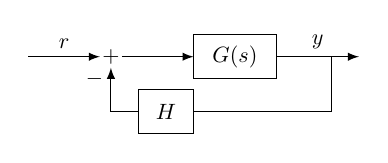
\begin{tikzpicture}[scale=0.7, every node/.style={scale=0.8}]
\node at (0,0) {$+$};
\draw[-latex] (-1.5,0) -- (-0.2,0) node[midway,above] {$r$};
\draw[-latex] (0.2,0) -- (1.5,0);
\draw (1.5,-0.4) rectangle (3,0.4);
\node at (2.25,0) {$G(s)$};
\draw[-latex] (3,0) -- (4.5,0) node[midway,above] {$y$};
\draw (4,0) -- (4,-1) -- (1.5,-1);
\draw (0.5,-1.4) rectangle (1.5,-0.6);
\node at (1,-1) {$H$};
\draw[-latex] (0.5,-1) -- (0,-1) -- (0,-0.2);
\node at (-0.3,-0.4) {$-$};
\end{tikzpicture}
\end{center}

\importantbox{
\begin{equation*}
G_{\text{closed}}(s) = \frac{G(s)}{1 + G(s)H(s)}
\end{equation*}
}

\subsection{Loop Gain}
\begin{equation*}
L(s) = G(s)H(s)
\end{equation*}
\begin{itemize}
\item $|L| \gg 1$: output $\approx r/H$ (feedback dominates)
\item $|L| \ll 1$: output $\approx G \cdot r$ (open loop)
\end{itemize}

\subsection{Feedback Effects}
\begin{center}
\begin{tabular}{ll}
\toprule
Property & Effect of Neg. Feedback \\
\midrule
Gain & Reduced by $(1+L)$ \\
Bandwidth & Increased \\
Disturbance rejection & Improved \\
Sensitivity to $G$ & Reduced \\
Stability & Can destabilize \\
\bottomrule
\end{tabular}
\end{center}

\subsection{Effect on Control Coefficients}
Negative feedback \textit{redistributes} control:
\begin{itemize}
\item Reduces control of feedback-regulated enzyme
\item Increases control of the enzyme beyond the signal
\item Total still sums to 1 (for flux)
\end{itemize}

% =============================================================================
\section{Perfect Adaptation}
% =============================================================================

\subsection{Definition}
Output returns to \textit{same} steady state regardless of sustained input change.

\subsection{Transfer Function Requirement}
\importantbox{
Perfect adaptation $\Leftrightarrow$ $G(0) = 0$
\vspace{3pt}

Requires a \textbf{zero at $s = 0$} in the transfer function
}

\subsection{Implementation: Integral Feedback}

Minimal system for perfect adaptation:
%
\begin{align*}
\frac{dY}{dt} &= k_a L - k_b M Y \\[4pt]
\frac{dM}{dt} &= k_1 Y - k_0
\end{align*}

\begin{itemize}
\item $L$ = input signal (perturbation here)
\item $Y$ = output (adapting variable)
\item $M$ = adaptation variable (integrator)
\item $k_0$ = constant removal of $M$ (zero-order)
\end{itemize}

\textbf{Steady-state analysis:}

From $dM/dt = 0$:
\begin{equation*}
Y^{ss} = \frac{k_0}{k_1} \quad \text{(independent of } L \text{)}
\end{equation*}

From $dY/dt = 0$:
\begin{equation*}
M^{ss} = \frac{k_a L}{k_b Y^{ss}} = \frac{k_a k_1}{k_b k_0} L
\end{equation*}

$M$ adjusts to absorb changes in $L$, keeping $Y$ at its setpoint.

\textbf{Key:} The constant $k_0$ (zero-order in $M$) makes $M$ a true integrator.

\subsection{The Integral Controller}
The integrator $\frac{1}{s}$ in the feedback path creates:
\begin{itemize}
\item A pole at $s=0$ in $H(s)$
\item A zero at $s=0$ in $G_{\text{closed}}(s)$
\item $\Rightarrow$ Perfect adaptation
\end{itemize}

\subsection{High-Pass Filter Behavior}
Perfect adaptation means:
\begin{itemize}
\item Low frequencies: attenuated ($|G| \to 0$)
\item High frequencies: pass through
\item System responds to \textit{changes}, ignores \textit{levels}
\end{itemize}

% =============================================================================
\section{Retroactivity}
% =============================================================================

\subsection{Definition}
When modules are connected, downstream modules \textit{load} upstream modules, changing their behavior.

%\subsection{Impedance Analogy}
%\begin{align*}
%Z_{\text{out}} &= \text{output impedance (source)} \\
%Z_{\text{in}} &= \text{input impedance (load)}
%\end{align*}
%Loading is small when $Z_{\text{in}} \gg Z_{\text{out}}$

\subsection{Insulation Strategies}
\begin{itemize}
\item High-gain cascades (like MAPK)
\item Phosphorylation cycles with fast kinetics - debatable
\item Enzymatic ``push-pull'' amplifiers
\end{itemize}

% =============================================================================
\section{Stability Analysis}
% =============================================================================

\subsection{Routh-Hurwitz (2nd Order)}
For $\Delta(s) = s^2 + as + b$:
\begin{itemize}
\item Stable iff $a > 0$ AND $b > 0$
\end{itemize}

\subsection{Routh-Hurwitz (3rd Order)}
For $\Delta(s) = s^3 + as^2 + bs + c$:
\begin{itemize}
\item Stable iff $a > 0$, $c > 0$, AND $ab > c$
\end{itemize}

\subsection{Hopf Bifurcation}
Oscillations emerge when complex eigenvalues cross imaginary axis:
\begin{itemize}
\item $\text{Re}(\lambda) = 0$, $\text{Im}(\lambda) = \omega \neq 0$
\item Oscillation period $T = 2\pi/\omega$
\end{itemize}

\subsection{Conditions for Oscillations}
\begin{enumerate}
\item Negative feedback (delayed)
\item Sufficient loop gain
\item Sufficient delay (or chain length)
\end{enumerate}

% =============================================================================
\section{Useful Identities}
% =============================================================================

\subsection{Matrix Inverse (2$\times$2)}
\begin{equation*}
\begin{pmatrix} a & b \\ c & d \end{pmatrix}^{-1} = \frac{1}{ad-bc}\begin{pmatrix} d & -b \\ -c & a \end{pmatrix}
\end{equation*}

\subsection{Complex Number Magnitude}
\begin{equation*}
|a + jb| = \sqrt{a^2 + b^2}
\end{equation*}

\subsection{Complex Number Phase}
\begin{equation*}
\angle(a + jb) = \arctan(b/a)
\end{equation*}

\subsection{Laplace Transform Pairs}
\begin{center}
\begin{tabular}{cc}
\toprule
$f(t)$ & $F(s)$ \\
\midrule
$e^{-at}$ & $\dfrac{1}{s+a}$ \\[8pt]
$1 - e^{-at}$ & $\dfrac{a}{s(s+a)}$ \\[8pt]
$te^{-at}$ & $\dfrac{1}{(s+a)^2}$ \\[8pt]
$\sin(\omega t)$ & $\dfrac{\omega}{s^2+\omega^2}$ \\[8pt]
step & $\dfrac{1}{s}$ \\
\bottomrule
\end{tabular}
\end{center}

\subsection{Final Value Theorem}
If $\lim_{t\to\infty} y(t)$ exists:
\begin{equation*}
\lim_{t\to\infty} y(t) = \lim_{s\to 0} s \cdot Y(s)
\end{equation*}

% =============================================================================
\section{Quick Reference: Tellurium}
% =============================================================================

\subsection{Basic Operations}
\begin{Verbatim}[fontsize=\scriptsize]
import tellurium as te
r = te.loada('''
  -> S; k1*L - k2*S
  S = 1; k1 = 1; k2 = 0.1; L = 1
''')

# Steady state
r.steadyState()

# Simulate
result = r.simulate(0, 100, 500)
\end{Verbatim}

\subsection{Stoichiometric Analysis}
\begin{Verbatim}[fontsize=\scriptsize]
# Full stoichiometry matrix N
N = r.getFullStoichiometryMatrix()

# Reduced stoichiometry matrix Nr
Nr = r.getReducedStoichiometryMatrix()

# Link matrix L
L = r.getLinkMatrix()

# Conservation matrix G (left null)
G = r.getConservationMatrix()

# Kernel matrix K (right null)
K = r.getKMatrix()
\end{Verbatim}

\subsection{MCA and Dynamics}
\begin{Verbatim}[fontsize=\scriptsize]
# Jacobian
A = r.getFullJacobian()

# Eigenvalues
import numpy as np
eigs = np.linalg.eigvals(J)

# Elasticities (scaled)
ee = r.getScaledElasticityMatrix()

# Control coefficients
ccJ = r.getScaledFluxControlCoefficientMatrix()
ccS = r.getScaledConcentrationControlCoefficientMatrix()
\end{Verbatim}

% =============================================================================
\section{Matrix Summary Table}
% =============================================================================

\begin{center}
\footnotesize
\begin{tabular}{lccp{2.2cm}}
\toprule
\textbf{Matrix} & \textbf{Size} & \textbf{Sym.} & \textbf{Meaning} \\
\midrule
Stoichiometry & $m \times r$ & $\mathbf{N}$ & Network structure \\
Reduced stoich. & $m_0 \times r$ & $\mathbf{N}_r$ & Indep.\ species \\
Link & $m \times m_0$ & $\mathbf{L}$ & Dep./indep.\ relation \\
Kernel & $r \times (r{-}m_0)$ & $\mathbf{K}$ & SS flux basis \\
Conservation & $(m{-}m_0) \times m$ & $\mathbf{G}$ & Conserved moieties \\
Elem.\ modes & $r \times n_{EM}$ & $\mathbf{E}$ & Minimal pathways \\
Elasticity & $r \times m$ & $\boldsymbol{\varepsilon}$ & Local kinetics \\
Jacobian & $m \times m$ & $\mathbf{A}$ & Dynamics \\
Control (flux) & $r \times r$ & $\mathbf{C}^J$ & Flux sensitivity \\
Control (conc.) & $m \times r$ & $\mathbf{C}^S$ & Conc.\ sensitivity \\
\bottomrule
\end{tabular}
\end{center}

\textbf{Key:} $m$ = species, $r$ = rxns, $m_0$ = rank($\mathbf{N}$)

\subsection{Fundamental Relationships}
\begin{align*}
\mathbf{N} &= \mathbf{L} \cdot \mathbf{N}_r & \mathbf{N} \cdot \mathbf{K} &= \mathbf{0} \\
\mathbf{G} \cdot \mathbf{N} &= \mathbf{0} & \mathbf{G} \cdot \mathbf{L} &= \mathbf{0} \\
\mathbf{J} &= \mathbf{N} \cdot \boldsymbol{\varepsilon}^u & \mathbf{C} \cdot \boldsymbol{\varepsilon} &= -\mathbf{I}
\end{align*}

\vfill
\hrule
\vspace{3pt}
\footnotesize
\textit{Advanced Control of Biochemical Networks.\\ Herbert M Sauro,} \today 

\end{multicols}
\end{document} 